\chapter{Manual de usuario de la aplicación}
\label{anx:manual}

La aplicación suministrada ofrece capacidades para la gestión de usuarios del servicio de \acf{WVD} creado y disponible en Azure para la organización correspondiente. Permite realizar tareas como consultar los diferentes \textit{hostpools} creados, así como las diferentes tareas que tienen que ver con los grupos de aplicaciones de estos: creación y eliminación de grupos, consulta de parámetros y modificación de aplicaciones y usuarios con acceso a estos. En las sucesivas secciones del presente manual se explicarán estas funcionalidades y la manera de proceder en cada una de ellas.

\section{Conexión a Azure}
La primera ventana que verá al iniciar la aplicación será la que se encarga de realizar la conexión a Azure (Figura \ref{fig:man_main_conex}). Como se observa, la aplicación muestra un único botón disponible llamado <<conectar a Azure>> que, al hacer clic sobre este, lanzará una nueva ventana emergente en la que se deberán introducir los datos correspondientes al usuario con acceso al servicio para su gestión. Dependiendo de la implementación del servicio de autenticación en cada organización, al introducir la dirección de correo en la página de Microsoft (Figura \ref{fig:man_inicio_microsoft}) se le redigirá a la página de autenticación de dicha organización que, a modo de ejemplo, se ilustra con la correspondiente a la de la \acf{UCLM} (Figura \ref{fig:man_inicio_uclm}).

\begin{figure}[h]
  \centering
  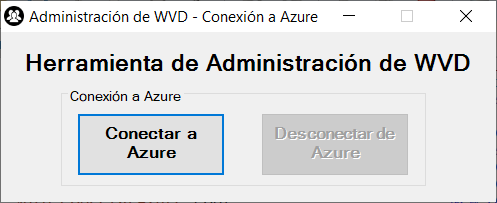
\includegraphics[width=0.7\linewidth]{figures/images/script/main_conex.PNG}
  \caption{Ventana de conexión a Azure}
  \label{fig:man_main_conex}
\end{figure}

\clearpage

\begin{figure}
    \centering
    \begin{minipage}{.5\textwidth}
        \centering
        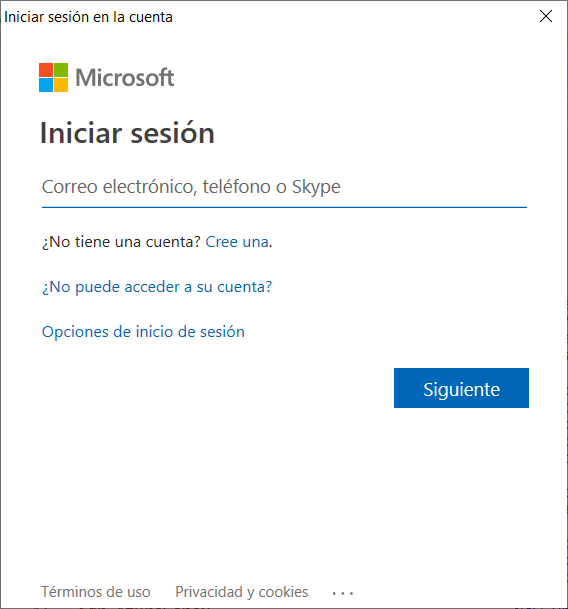
\includegraphics[width=0.8\linewidth]{figures/images/script/inicio_microsoft.PNG}
        \caption{Inicio de sesión en Microsoft}
        \label{fig:man_inicio_microsoft}
    \end{minipage}%
    \begin{minipage}{.5\textwidth}
        \centering
        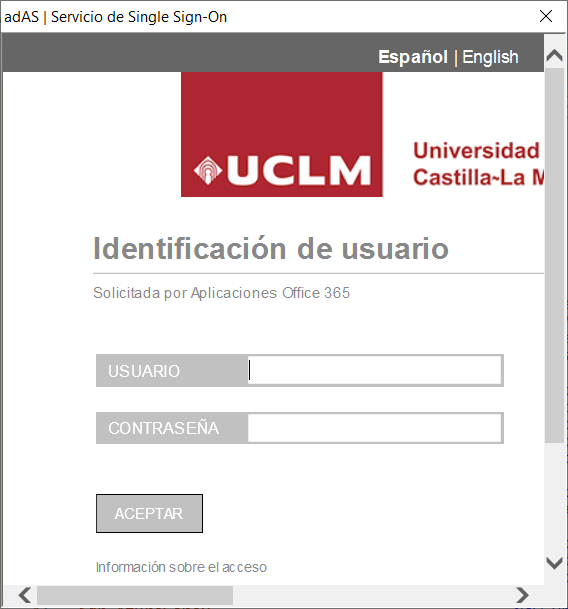
\includegraphics[width=0.8\linewidth]{figures/images/script/inicio_uclm.PNG}
        \caption{Inicio de sesión en la \acs{UCLM}}
        \label{fig:man_inicio_uclm}
    \end{minipage}
\end{figure}

Si el proceso de autenticación se ha realizado correctamente, se le avisará mediante un mensaje en una ventana de información. Lo mismo ocurrirá en caso contrario. En el supuesto de que la autenticación se haya realizado sin errores, la ventana mostrada en la Figura \ref{fig:man_main_conex} se expandirá mostrando más elementos (Figura \ref{fig:man_main_expand}). En primer lugar, el botón <<conectar a Azure>> se encuentra deshabilitado, mientras que el botón <<desconectar de Azure>> se habrá habilitado. Esto representa que la sesión en Azure ha sido establecida y será posible cerrarla para volver al primer paso. En los campos <<App ID>> y <<Password>> se deberán escribir las credenciales correspondientes al servicio de \acs{WVD} enlazadas con la dirección de correo que se ha utilizado previamente para iniciar sesión en Azure. De igual manera, tanto si la identificación en el servicio se ha realizado correctamente como si ha ocurrido algún error, se avisará mediante un mensaje en una ventana emergente. Una vez identificado en el servicio, la ventana actual se cerrará para acceder al menú principal, desde donde se pueden realizar todas las acciones.

\begin{figure}[h]
  \centering
  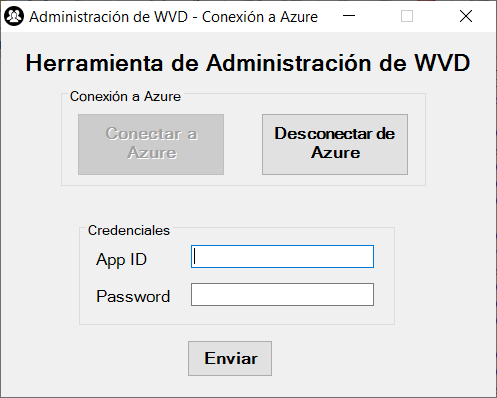
\includegraphics[width=0.5\linewidth]{figures/images/script/main_expand.PNG}
  \caption{Ventana de conexión al servicio de \acs{WVD}}
  \label{fig:man_main_expand}
\end{figure}

\section{Consultar información de \textit{hostpools}}
Desde el menú principal (Figura \ref{fig:man_menu_ppal}), es posible realizar consultas para obtener información acerca de los \textit{hostpools} disponibles en el servicio. Para ello, haga clic en el botón <<ver \textit{hostpools} disponibles>> y seleccione el \textit{hostpool} de entre los disponibles en la lista desplegable que se mostrará en la parte superior de una nueva ventana, como se ilustra en la Figura \ref{fig:man_info_hostpools}. Una vez realizados estos pasos y la información sea cargada en cada uno de los campos, será posible consultar los diferentes parámetros de los \textit{hostpools} que se encuentran creados en el servicio.

\begin{figure}[h]
  \centering
  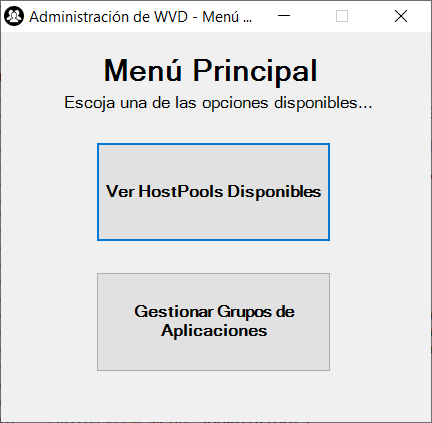
\includegraphics[width=0.6\linewidth]{figures/images/script/menu_ppal.PNG}
  \caption{Menú principal}
  \label{fig:man_menu_ppal}
\end{figure}

\begin{figure}[h]
  \centering
  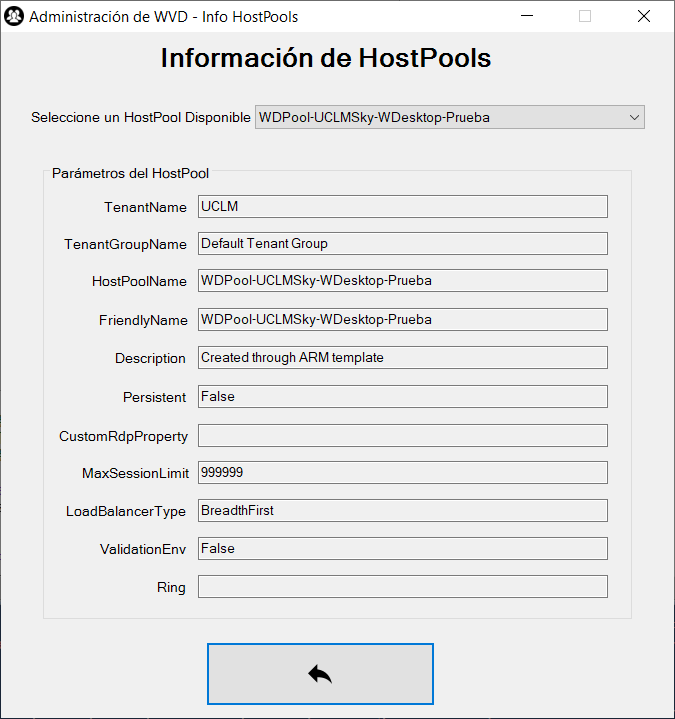
\includegraphics[width=0.8\linewidth]{figures/images/script/info_hostpools.PNG}
  \caption{Ventana de información de \textit{hostpools}}
  \label{fig:man_info_hostpools}
\end{figure}

\clearpage

\section{Gestionar grupos de aplicaciones}
La otra funcionalidad principal de esta aplicación es la de poder gestionar los diferentes grupos de aplicaciones. Estos grupos contendrán tanto aplicaciones como usuarios a los que se otorgue acceso y que podrán hacer uso de las mismas. La ventana desde la que se pueden realizar las acciones relativas a estos se muestra en la Figura \ref{fig:man_ventana_gestion}.  A continuación, se detallarán los procedimientos que se pueden llevar a cabo utilizando la aplicación con respecto a dichos grupos.

\begin{figure}[h]
  \centering
  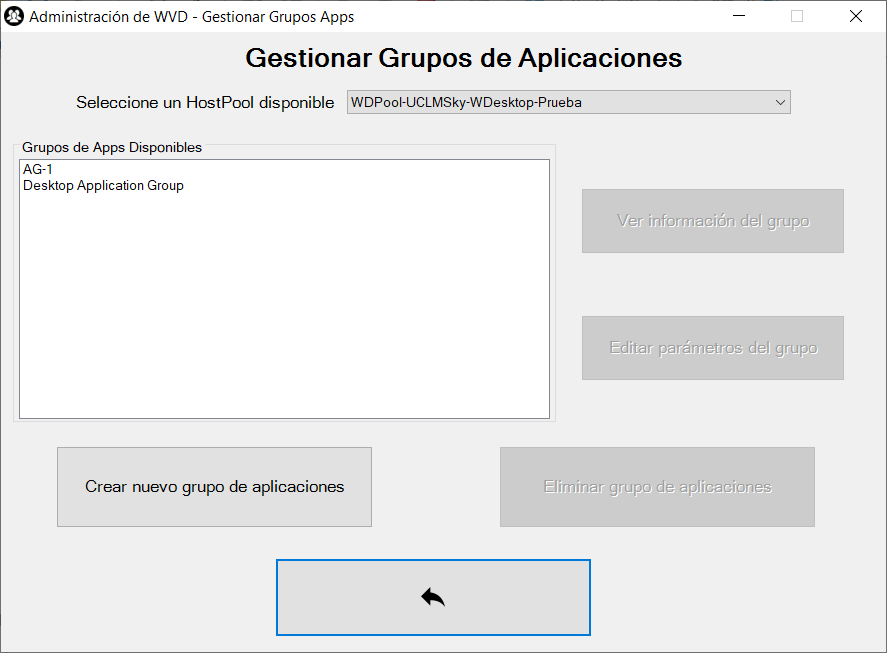
\includegraphics[width=0.9\linewidth]{figures/images/script/ventana_gestion.PNG}
  \caption{Ventana de gestión de grupos}
  \label{fig:man_ventana_gestion}
\end{figure}

\clearpage

\subsection{Crear un nuevo grupo de aplicaciones}
Para crear un nuevo grupo de aplicaciones, haga clic sobre el botón <<gestionar grupos de aplicaciones>> en el menú principal y seleccione el \textit{hostpool} sobre el que desea operar en la ventana que se muestra. A continuación, pulse sobre el botón <<crear nuevo grupo de aplicaciones>> y rellene los parámetros que se solicitan en la ventana emergente (Figura \ref{fig:man_ventana_creargrupo}). Dependiendo del propósito del grupo de aplicaciones, puede seleccionar dos tipos de recursos:

\begin{itemize}
    \item \textbf{\textit{RemoteApp}}. Este tipo de recursos se encuentra enfocado a ofrecer únicamente aplicaciones individuales a los usuarios con acceso.
    
    \item \textbf{\textit{Desktop}}. En lugar de ofrecer aplicaciones individuales, este tipo de recursos ofrecerá a los usuarios un escritorio virtual completo, con todas las aplicaciones disponibles que se encuentren instaladas en ese \textit{hostpool}.
\end{itemize}

Finalmente, al pulsar sobre <<crear grupo>>, se informará si se ha creado correctamente el nuevo grupo y se mostrará este en la lista de grupos de aplicaciones disponibles.

\begin{figure}[h]
  \centering
  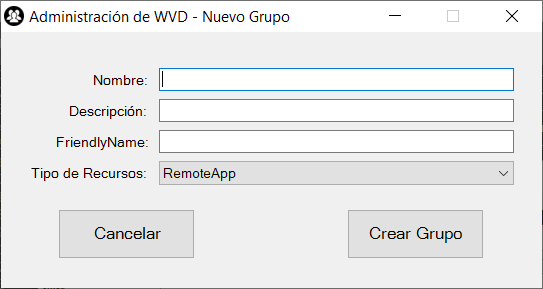
\includegraphics[width=0.7\linewidth]{figures/images/script/ventana_creargrupo.PNG}
  \caption{Ventana de creación de grupo}
  \label{fig:man_ventana_creargrupo}
\end{figure}


\subsection{Eliminar un grupo de aplicaciones existente}
De igual manera que se ofrece la posibilidad de crear un nuevo grupo, es posible llevar a cabo su eliminación del servicio. Para realizar esta tarea, seleccione de la lista que se muestra el que se desea eliminar y pulse sobre el botón <<eliminar grupo de aplicaciones>>. Se mostrará una confirmación que, de ser positiva, desencadenará la eliminación del grupo seleccionado, desapareciendo de la lista.

\clearpage

\subsection{Consultar información de un grupo de aplicaciones}
Es posible consultar toda la información de los grupos de aplicaciones sin poder realizar cambios para evitar modificaciones indeseadas. Para ello, seleccione un grupo de entre los disponibles y pulse sobre el botón <<ver información del grupo>> o haga doble clic sobre el grupo deseado. Esto abrirá una nueva ventana en la que se mostrará la información acerca de los parámetros del grupo, las aplicaciones disponibles y los usuarios con acceso al mismo. La Figura \ref{fig:man_ventana_infogrupo} muestra la información de un grupo cuyo tipo de recursos es <<RemoteApp>>. En el caso de que este parámetro sea <<Desktop>>, en la lista de aplicaciones se mostrará un único elemento indicando que ese tipo de grupo no es compatible con la selección de aplicaciones (Figura \ref{fig:man_ventana_infogrupoDesktop}).

\begin{figure}[h]
  \centering
  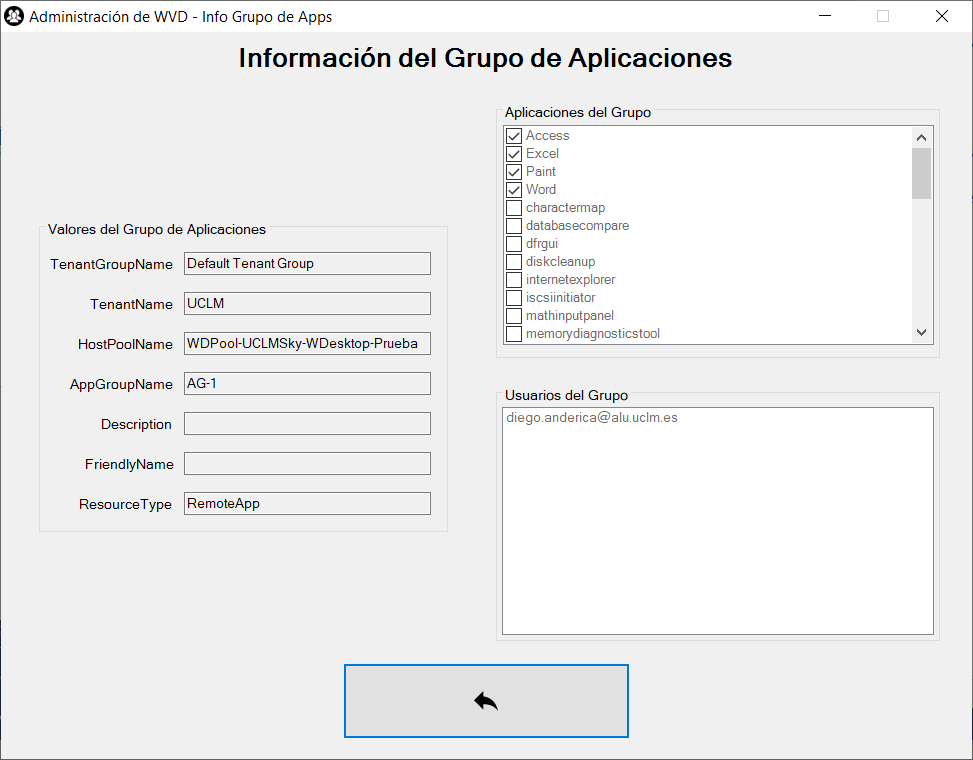
\includegraphics[width=0.8\linewidth]{figures/images/script/ventana_infogrupo.PNG}
  \caption{Ventana de información de grupo}
  \label{fig:man_ventana_infogrupo}
\end{figure}

\begin{figure}[h]
  \centering
  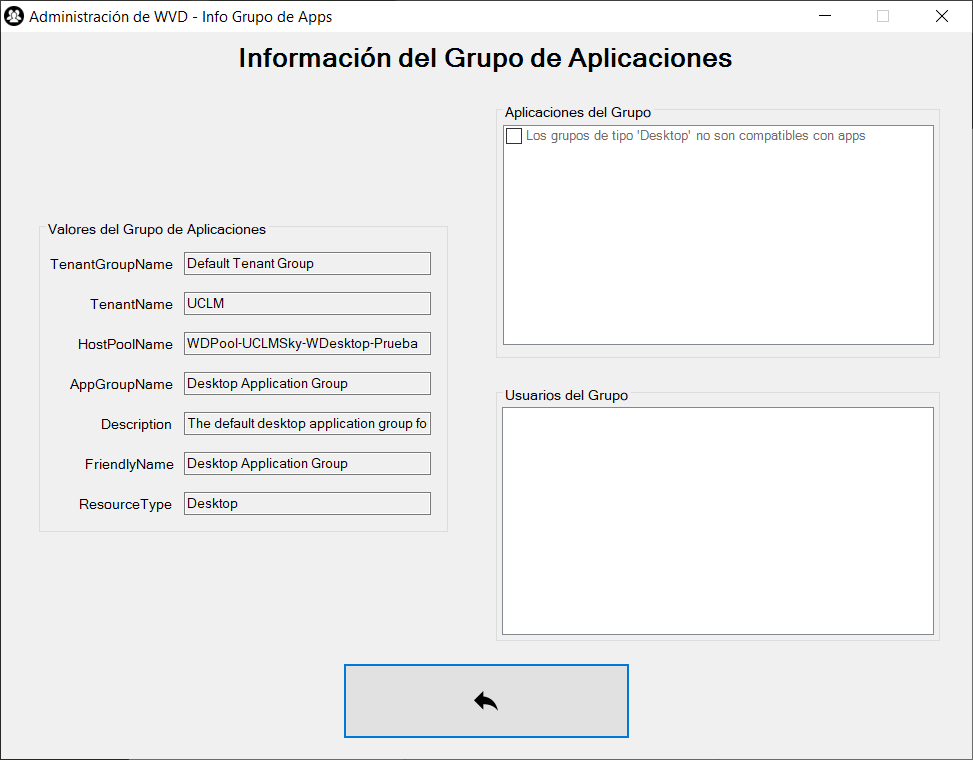
\includegraphics[width=0.8\linewidth]{figures/images/script/ventana_infogrupoDesktop.PNG}
  \caption{Ventana de información de grupo (\textit{ResourceType Desktop})}
  \label{fig:man_ventana_infogrupoDesktop}
\end{figure}

\clearpage

\subsection{Editar aplicaciones y usuarios de un grupo de aplicaciones}
Para modificar las aplicaciones disponibles y los usuarios con acceso a un grupo de aplicaciones, siga las indicaciones que se detallan a continuación. La ventana sobre la que se centrarán estas se muestra en la Figura \ref{fig:man_ventana_editargrupo} donde, además, es posible consultar los valores de los parámetros que se especificaron en el momento de creación del grupo en la parte izquierda de la ventana.

\begin{figure}[h]
  \centering
  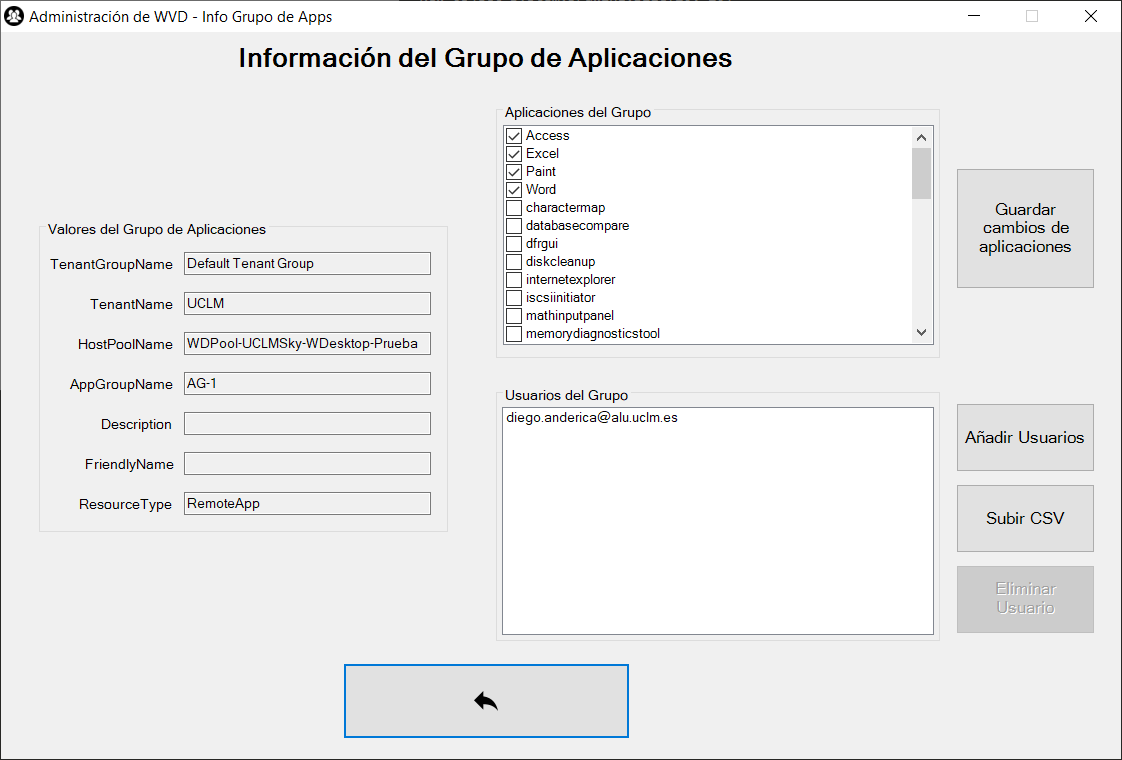
\includegraphics[width=0.8\linewidth]{figures/images/script/ventana_editargrupo.PNG}
  \caption{Ventana de edición de grupo}
  \label{fig:man_ventana_editargrupo}
\end{figure}

\subsubsection{Editar aplicaciones de un grupo de aplicaciones}
Si desea editar las aplicaciones que se ofrecerán dentro de un grupo de aplicaciones, seleccione sobre el que se desea editar en la lista y haga clic sobre el botón <<editar parámetros del grupo>>. A continuación, marque o desmarque las aplicaciones que desea que sean entregadas y pulse sobre el botón <<guardar cambios de aplicaciones>>. Después de confirmar la acción y de que la aplicación recargue la correspondiente información, los cambios serán mostrados en la correspondiente lista.

\clearpage

\subsubsection{Añadir usuarios a un grupo de aplicaciones}
También es posible editar la lista de los usuarios con acceso a un grupo de aplicaciones. Es posible realizar esta gestión de dos maneras diferentes: introduciendo usuarios a mano o a través de un archivo \acs{CSV}. En el caso de que se introduzcan a mano, pulse sobre el botón <<añadir usuarios>> y escriba en la ventana emergente (Figura  \ref{fig:man_ventana_addUsuarios}) las direcciones de correo de los usuarios a los que se desea otorgar acceso. Puede escribir una única dirección o un conjunto de direcciones separadas por comas.

\begin{figure}[h]
  \centering
  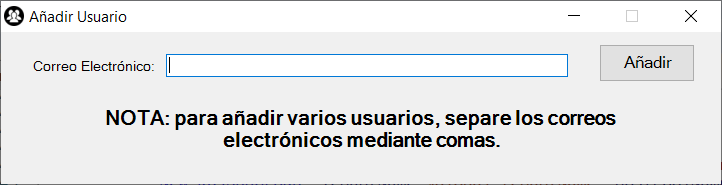
\includegraphics[width=0.8\linewidth]{figures/images/script/addUsuario.PNG}
  \caption{Ventana para añadir usuarios}
  \label{fig:man_ventana_addUsuarios}
\end{figure}

Como se ha mencionado anteriormente, también es posible añadir usuarios a un grupo de aplicaciones a través de un archivo \acs{CSV} pulsando sobre el botón <<subir \acs{CSV}>>. El formato de el archivo que se utilice tendrá las siguientes restricciones:

\begin{itemize}
    \item \textbf{Extensión}: *.csv.
    \item \textbf{Carácter de separación de valores}: <<;>> (punto y coma).
    \item \textbf{Campos}: Indiferente, siempre y cuando haya un campo <<Correo>> en la especificación de valores en la primera línea del archivo.
\end{itemize}

Al seleccionar un archivo válido el programa le avisará de que, si desea continuar, se borrarán todos los usuarios existentes para tener en cuenta únicamente los especificados en dicho archivo. De esta manera, se evitan redundancias y se asegura que el grupo se encuentra únicamente disponible para el conjunto especificado de usuarios, puesto que se considera que el archivo contiene todos los valores requeridos y necesarios para ofrecer el servicio a unos determinados usuarios.

\subsubsection{Eliminar un usuario de un grupo de aplicaciones}
Por último, es posible revocar el acceso de un usuario a un grupo determinado de aplicaciones. En este caso, bastará con seleccionar la dirección de correo deseada de la lista y hacer clic sobre el botón <<eliminar usuario>>. Tras realizar esta acción, el programa pedirá su confirmación y realizará la acción, recargando la lista correspondiente.